\section{Teoría de Conjuntos}
Hasta ahora hemos usado conjuntos y varios conceptos relacionados de una manera intuitiva pero razonable.
En esta sección estudiaremos la Teoría de Conjuntos desde un punto de vista axiomático, esta teoría se considera la base de las matemáticas.

La noción intuitiva nos dice que un \emph{conjunto} es una colección bien definida de objetos.
Estos objetos se llaman \emph{elementos} del conjunto y se dice que \emph{pertenecen} a él.
Ninguna de las anteriores son definiciones formales, en ella aparecen tres conceptos indispensables en la teoría:
\begin{itemize}
\itemsep 0pt
\item conjunto
\item elemento
\item pertenencia (que denotaremos por $\in$)
\end{itemize}
No daremos una explicación mas detallada de estos conceptos y apelaremos a la intuición para poder manejarlos.
Sólo notaremos que en la ``semi--definición'' de elemento usamos la palabra \emph{objeto}, refiriéndonos a ``cualquier cosa''.

Por ejemplo si escribimos
\[
x\in A\;\;\;\;\;\;\;\;\;\;1\in\N\;\;\;\;\;\;\;\;\;\;2\in\{1,2\}\in\{\{1,2\}\{2,3\}\}
\]
leeremos ``$x$ pertenece a $A$'' o ``$x$ es un elemento de $A$'', ``$1$ pertenece a los naturales'' (asumiendo que estamos de acuerdo en la notación), y que ``$2$ es un elementos de $\{1,2\}$ el que a su vez es un elemento de $\{\{1,2\},\{2,3\}\}$''.
Este último ejemplo puede resultar confuso pero no debe resultar contradictorio, nuestra ``semi--definición'' de elemento no impide para nada que un conjunto pueda ser un elemento de otro conjunto, de hecho todos los elementos de $\{\{1,2\},\{2,3\}\}$ son conjuntos.

\subsubsection*{Axioma de Extensión}
>Cuándo dos conjuntos son iguales?
Necesitamos un par de definiciones para responder esta pregunta.

\begin{definicion}
Sean $A$ y $B$ conjuntos, diremos que $A$ es subconjunto de $B$ y escribiremos $A\subseteq B$ si
\[
\text{ para todo } x \text{ se tiene que si }x\in A\text{ entonces }x\in B.
\]
%o sea, $A$ es subconjunto de $B$ si cada elemento de $A$ está también en $B$.
\end{definicion}

Por ejemplo, algunas relaciones como $\N\subseteq\Z$, o $\{1,2\}\subseteq\{1,2,3\}$ se cumplen.
Note que $\{1,2\}\not\subseteq\{\{1,2\},\{2,3\}\}$.

\begin{definicion}
Sean $A$ y $B$ conjuntos, diremos que $A$ y $B$ son iguales ($A=B$) si se cumplen simultáneamente:
\[
\begin{array}{c}
A\subseteq B\\
B\subseteq A,
\end{array}
\]
\end{definicion}

La anterior definición nos dice que dos conjuntos son iguales cuando tienen exactamente los mismos elementos.
De inmediato esta definición nos lleva a concluir que $\{x,x\}=\{x\}$ (ambos tienen exactamente a $x$ como elemento) y que por lo tanto los conjuntos no pueden tener elementos repetidos (o al menos no tiene ningún sentido que repitamos elementos en un conjunto). 
A la anterior definición se le llama comúnmente \emph{Axioma de Extensión} y puede formularse como que un conjunto queda completamente definido por los elementos que contiene.

\subsubsection*{Axioma del Conjunto Vacío}
A pesar de que nuestra teoría parte de nociones primitivas intuitivas, podemos establecer ciertos puntos de partida mas formales.
El primero es establecer la existencia de un conjunto.
El \emph{Axioma del Conjunto Vacío} nos habla de la existencia de un conjunto, nos dice que existe un conjunto que no tiene elemento alguno:
\[
\text{ existe un conjunto }X\text{ tal que para todo }x\text{ se tiene que }x\notin X.
\]
A ese conjunto lo llamaremos ``conjunto vacío'' y lo denotaremos por $\emptyset$ o simplemente $\{\}$.
Existen varias propiedades del conjunto vacío, las dos más importantes las establecemos en el siguiente teorema:

\begin{teorema}
	Las siguientes son propiedades del conjunto vacío:
	\begin{enumerate}
	  \vspace*{-\topsep}
	  \itemsep 0pt
		\item Para todo conjunto $A$ se tiene que $\emptyset\subseteq A$.
		\item Existe un único conjunto vacío.		
	\end{enumerate}
	
	\begin{demostracion}
	\begin{enumerate}
	  \vspace*{-\topsep}
	  \itemsep 0pt
		\item Tenemos que demostrar que $\forall x(x\in\emptyset\Rightarrow x\in A)$.
		La proposición ``$x\in\emptyset$'' es siempre falsa por lo tanto la implicación $x\in\emptyset\Rightarrow x\in A$ es siempre verdadera.
		Con palabras podríamos decirlo de la siguiente manera: queremos demostrar que el conjunto vacío es subconjunto de $A$, para esto tenemos que demostrar que todo elemento que está en el conjunto vacío está también en $A$, esto es trivialmente cierto ya que es una propiedad acerca de ``todos los elementos'' del conjunto vacío, y dado que no existen tales elementos, no hay nada que demostrar.
		\item Para demostrar unicidad en general lo que se hace es una demostración por contradicción suponiendo que existen dos objetos de los que se quiere demostrar que son únicos.
		Supongamos entonces que existen dos conjuntos vacíos $\emptyset_1$ y $\emptyset_2$ tales que $\emptyset_1\not=\emptyset_2$.
		Por la propiedad anterior, y dado que tanto $\emptyset_1$ como $\emptyset_2$ son conjuntos, se tiene que $\emptyset_1\subseteq\emptyset_2$, ya que estamos suponiendo que $\emptyset_1$ es vacío.
		Reciprocamente se tiene que $\emptyset_2\subseteq\emptyset_1$.
		Luego tenemos que $\emptyset_1\subseteq\emptyset_2$ y $\emptyset_2\subseteq\emptyset_1$ de lo que se deriva que $\emptyset_1=\emptyset_2$ que contradice la existencia de dos conjuntos vacíos distintos.
	\end{enumerate}
	\end{demostracion}
\end{teorema}

\subsubsection*{Pseudo--Axioma de Abstracción (Paradoja de Russell)}
>De qué manera podemos definir un conjunto?
Una manera inicial es la definición \emph{por extensión} es decir, listando cada uno de sus elementos, por ejemplo:
\[
\Z_5=\{0,1,2,3,4\}.
\]
Podemos también usar maneras más \emph{comprensivas} como la siguiente:
\[
\Z_5=\{x\;|\;x\in\N\text{ y } x<5\}.
\]
El \emph{Axioma de Abstracción} nos permite definir un conjunto usando cualquier propiedad ``que se nos ocurra'', o sea podemos definir el conjunto $A=\{x\;|\;\varphi(x)\}$ para cualquier propiedad $\varphi$, $A$ sería entonces el conjunto de todos los elementos que cumplen $\varphi$
\[
x\in A\Leftrightarrow\varphi(x).
\]
Esta noción nos indica que a cada propiedad le corresponde un conjunto.

\begin{ejemplo}
>Cómo podríamos definir el conjunto vacío usando este axioma?
Simplemente encontrando una propiedad  que ningún elemento cumpla.
Una posible propiedad sería
\[
\varphi(x)\Leftrightarrow x\not=x.
\]
Es claro que no existe ningún $x$ que cumpla esta propiedad, luego el conjunto
\[
\{x\;|\;x\not=x\}
\]
es vacío, o sea, $\emptyset=\{x\;|\;x\not=x\}$.
\end{ejemplo}
Este axioma es bastante ``permisivo'' en el sentido de que su formulación nos permite usar {\bf cualquier} propiedad, entre las que podrían encontrarse:
\begin{itemize}
	\vspace*{-\topsep}
	\itemsep 0pt
	\item[] $\varphi_1(x)$: $x$ es un conjunto con más de $3$ elementos
	\item[] $\varphi_2(x)$: $x$ es un conjunto con una cantidad finita de elementos
	\item[] $\varphi_3(x)$: $x$ es un conjunto con una cantidad infinita de elementos ($\varphi_3(x)\Leftrightarrow\neg\varphi_2(x)$)
\end{itemize}
para las cuales existirían conjuntos
\begin{itemize}
	\vspace*{-\topsep}
	\itemsep 0pt
	\item[] $\A_1=\{x\;|\;\varphi_1(x)\}$ el conjunto de todos los conjuntos con más de $3$ elementos
	\item[] $\A_2=\{x\;|\;\varphi_2(x)\}$ el conjunto de todos los conjuntos con una cantidad finita de elementos
	\item[] $\A_3=\{x\;|\;\varphi_3(x)\}$ el conjunto de todos los conjuntos con una cantidad infinita de elementos.
\end{itemize}
Ahora, nos podemos hacer la siguiente pregunta acerca de $\A_1$: dado que $\A_1$ es un conjunto que tiene conjuntos adentro, >Es $\A_1$ un elemento de si mismo? >$\A_1\in \A_1$?
En $\A_1$ se encuentran todos los conjuntos que tienen más $3$ elementos, de inmediato notamos que en $\A_1$ existen muchísimos conjuntos y que por lo tanto el mismo $\A_1$ tiene más de $3$ elementos, luego $\A_1$ cumple $\varphi_1$ y por lo tanto $\A_1\in \A_1$.
Si nos preguntamos lo mismo acerca de $\A_2$ llegamos a la conclusión de que $\A_2\notin \A_2$ esto porque en $\A_2$ están sólo los conjuntos con una cantidad finita de elementos, sin embargo $\A_2$ tiene una cantidad infinita de elementos (existen infinitos conjuntos con una cantidad finita de elementos), por lo que $\A_2$ no cumple $\varphi_2$ y por lo tanto $\A_2\notin \A_2$.
Con una argumentación similar a las anteriores nos damos cuenta que $\A_3$ cumple con $\varphi_3$ y que por lo tanto $\A_3\in \A_3$.

Por la discusión notamos que tiene sentido preguntarse si un conjunto cualquiera pertenece o no a sí mismo.
Podríamos tomar entonces la siguiente propiedad:
\[
\varphi(x)\Leftrightarrow x\notin x,
\]
o sea, $\varphi$ la cumplen todos los conjuntos que no pertenecen a sí mismos.
Usando los ejemplos anteriores, $\A_2$ cumple $\varphi$ mientras que $\A_1$ y $\A_3$ no la cumplen. 

Según el Axioma de Abstracción existiría entonces un conjunto, llamémoslo $\mathcal{R}$ que se forma con todos los conjuntos $x$ que cumplen $\varphi(x)$, o sea, con todos los conjuntos que no son elementos de sí mismos:
\[
\mathcal{R}=\{x\;|\;x\notin x\}
\]
Ahora podríamos formularnos la siguiente pregunta:
¿Es $\mathcal{R}$ un elemento de $\mathcal{R}$? ¿$\mathcal{R}\in\mathcal{R}$?
El conjunto $\mathcal{R}$ pertenece a sí mismo si y sólo si cumple la propiedad $\varphi$, es decir, sólo si cumple con $\mathcal{R}\notin\mathcal{R}$.
Obtenemos lo siguiente:
\[
\mathcal{R}\in\mathcal{R}\Leftrightarrow\mathcal{R}\notin\mathcal{R}
\]
o sea, $\mathcal{R}$ pertenece a sí mismo si y sólo si $\mathcal{R}$ no pertenece a sí mismo... <Una contradicción en la matemática!
Esta contradicción se conoce como la \emph{paradoja de Russell} y fué descubierta por Bertrand Russell (1872--1970) en el año 1901.

\begin{nota}

\begin{figure}[h!]
	\begin{center}
	\begin{tabular}{cc}
	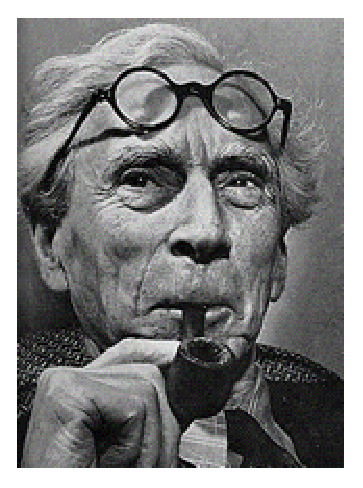
\includegraphics[width=140pt]{eps_imgs/russell.eps} \hspace*{30pt} &
	\hspace*{30pt} 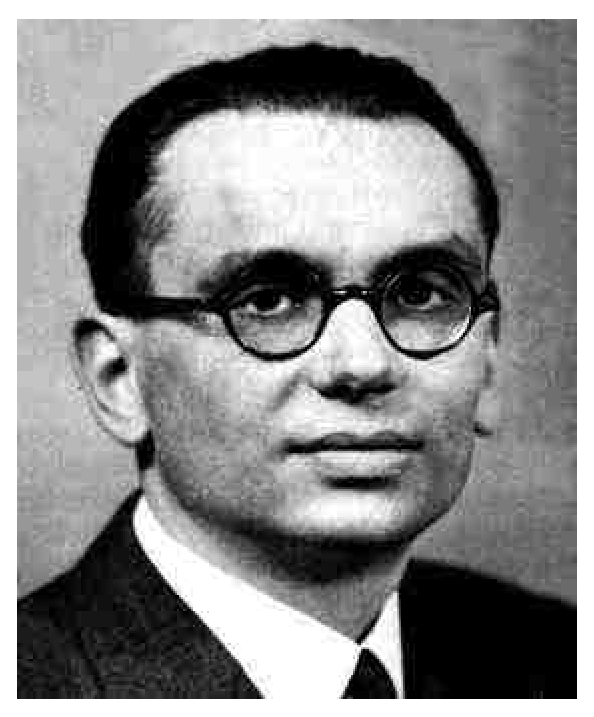
\includegraphics[width=150pt]{eps_imgs/godel.eps}
	\end{tabular}
	\end{center}
	\caption[]{Bertrand Russell 1872--1970 (izquierda), Kurt G\"odel 1906--1978 (derecha).}
\end{figure}

Russell fué un filósofo y matemático inglés y es conocido principalmente por sus aportes en lógica matemática y filosofía analítica.
Russell descubrió su paradoja justo cuando el matemático alemán Gottlob Frege (1848--1925) terminaba de escribir el segundo tomo de su libro \emph{The Basic Laws of Arithmetic} que pretendía dictar las pautas de la matemática en ese momento.
La paradoja de Russell puso en jaque el trabajo de Frege, principalmente porque en este se tomaba el axioma de abstracción como base para la construcción de conjuntos y por lo tanto se basaba en un hecho matemático contradictorio, lo que desmoronaba completamente la teoría.
La paradoja de Russell llegó a manos de Frege en el momento en que su libro ya se encontraba en la imprenta para ser publicado.
Frege debió entonces abortar la publicación y agregar un capítulo final a su libro sólo para intentar lidiar con la paradoja de Russell.
\end{nota}

>Dónde está el problema?
Principalmente por el hecho de considerar ``conjuntos muy grandes'' o ``colecciones de demasiados elementos''.
Esto es posible gracias a lo permisivo del axioma de abstracción.
La moraleja es que no cualquier propiedad puede ser tomada para crear un conjunto, en particular la propiedad $\varphi(x)\Leftrightarrow x\notin x$ no es una propiedad válida para crear un conjunto.

\subsubsection*{Axioma de Separación}
El axioma de abstracción es desechado por el hecho de que lleva a una contradicción.
Para reemplazarlo existe el \emph{Axioma de Separación}.
Este nos dice que para crear un conjunto, podemos usar una propiedad cualquiera pero sólo acerca de elementos que existen ya en otro conjunto que ha si creado ``sanamente''.
Con ``sanamente'' nos referimos a conjuntos que no han sido creados a partir del axioma de abstracción.
Con esto, podemos afirmar que, si $\varphi$ es una propiedad y $C$ es un conjunto entonces
\[
A=\{x\;|\;x\in C\text{ y }\varphi(x)\}
\]
también es un conjunto.
El conjunto $A$ se forma entonces \emph{separando} de $C$ los elementos que cumplen $\varphi$.

En el resto de estos apuntes muchas veces definiremos conjuntos usando simplemente una propiedad, en esos casos se supondrá que los elementos los estamos tomando de un conjunto ``universal sano'' que llamaremos $\mathcal{U}$, así cuando nos refiramos al conjunto $A=\{x\;|\;\varphi(x)\}$ realmente nos estaremos refiriendo a
\[A=\{x\;|\;x\in\mathcal{U}\text{ y }\varphi(x)\}.
\]

\begin{nota}
Estos axiomas, junto a otros (Axioma de Pares, de Uniones, del Conjunto Potencia, de Regularidad, de Reemplazo) que no enunciaremos pero veremos desde un punto de vista intuitivo, forman la base de la teoría de conjuntos.

El Axioma de Separación, evita la paradoja o contradicción de Russell que surgía ante el Axioma de Abstracción, la pregunta que uno podría hacerse es mayor,
>son los axiomas libres de otras contradicciones? 
>está la matemática (teoría de conjuntos) libre de contradicciones?
>es posible demostrar que no hay contradicciones en la matemática?
En cuanto a las primeras dos preguntas, hasta hoy no hay contradicciones conocidas, si las hubiera no tendría sentido estudiar esta teoría.
En cuanto a la última pregunta la respuesta es increíblemente NO, no es posible demostrar la consistencia (libertad de contradicción) de la matemática dentro de la matemática, o sea, la matemática no puede demostrar su propia consistencia.
Esta respuesta la dio el matemático Kurt G\"{o}del (1906--1978) en el año 1933.
Kurt G\"odel junto a Bertrand Russell son considerados los lógicos matemáticos mas importantes del siglo XX.

\end{nota}

\subsubsection*{Operaciones}
A partir de conjuntos dados es posible crear nuevos conjuntos aplicando operaciones entre ellos.
Sean $A$ y $B$ conjuntos, entonces las siguientes son operaciones elementales y el resultado de cada una es un conjunto\footnote{Aquí introduciremos una notación que esperamos se mantenga durante el desarrollo de los apuntes. En general para los elementos de conjuntos usaremos letras minúsculas como $x$, $y$ o $z$, para los conjuntos usaremos letras mayúsculas como $A$, $B$, o $C$ y para los conjuntos cuyos elementos son conjuntos usaremos letras cursivas como $\mathcal{R}$, $\mathcal{S}$ o $\mathcal{T}$.}:
\begin{itemize}
  \itemsep 0pt
  \item Unión: $A\cup B=\{x\;|\;x\in A\text{ o } x\in B\}$, los elementos que están en $A$ o en $B$.
  \item Intersección: $A\cap B=\{x\;|\;x\in A\text{ y } x\in B\}$, los elementos que simultáneamente están en $A$ y en $B$.
  \item Diferencia: $A\setminus B=\{x\;|\;x\in A\text{ y } x\notin B\}$, los elementos que están en $A$ pero no en $B$. 
  A veces escribiremos simplemente $A-B$ refiriéndonos a la diferencia de conjuntos.
  %\item Singleton: $\mathcal{S}(A)=\{A\}$, el conjunto que sólo tiene a $A$ como conjunto.
  \item Conjunto Potencia: $\P(A)=\{X\;|\;X\subseteq A\}$, el conjunto de todos los subconjuntos de $A$.
\end{itemize}

Estas operaciones ya debieran ser familiares para el alumno.
De ellas, tal vez el concepto más interesante es el del conjunto potencia, nótese que si $A$ es un conjunto cualquiera, entonces siempre se cumple que $\emptyset\in\P(A)$ y que $A\in\P(A)$ (>por qué?).
Otras propiedades que satisfacen estas operaciones son por ejemplo que para todos los conjuntos $A$ y $B$ se tiene que $A\subseteq A\cup B$ y que $A\cap B\subseteq A$.

\begin{ejemplo}[Construcción de los Naturales.]
Hasta ahora el único conjunto que sabemos con certeza que existe es el conjunto vacío $\emptyset$.
A partir de él podemos generar otros conjuntos usando el siguiente operador:
\[
\sigma(x)=x\cup\{x\}.
\]
Con el podríamos inductivamente hacer la siguiente construcción:
\[
\begin{array}{rcll}
0 & = & \emptyset \\
1 & = & \sigma(\emptyset) = \sigma(0) = \sigma(\emptyset) = \emptyset\cup\{\emptyset\} = \{\emptyset\} = \{0\}\\
2 & = & \sigma(\sigma(\emptyset)) = \sigma(1) = \sigma(\{\emptyset\}) = \{\emptyset\}\cup\{\{\emptyset\}\} = \{\emptyset,\{\emptyset\}\} = \{0,1\} \\
3 & = & \sigma(\sigma(\sigma(\emptyset))) = \sigma(2) = \sigma(\{\emptyset,\{\emptyset\}\}) = \{\emptyset,\{\emptyset\}\}\cup\{\{\emptyset,\{\emptyset\}\}\} = \{\emptyset,\{\emptyset\},\{\emptyset,\{\emptyset\}\}\} = \{0,1,2\}\\
%4 & = & \;\;\;\;\;\;\;\; \cdots \;\;\;\;\;\;\;\; = \{0,1,2,3\}\\
\vdots
\end{array}
\]
El operador $\sigma$ puede considerarse como el operador \emph{sucesor}, así el {\bf conjunto sucesor} de un conjunto $N$ es $\sigma(N)$.
La idea de esta construcción es que al conjunto vacío le llamamos $0$, al conjunto sucesor del conjunto vacío, o sea $\sigma(\emptyset)$, le llamamos $1$, al conjunto sucesor del conjunto sucesor del conjunto vacío, o sea $\sigma(\sigma(\emptyset))$, le llamamos $2$ y así continuamos hasta crear todos los naturales.

Con esto mostramos que la simple existencia del conjunto vacío basta para crear a todos los naturales, partiendo de que al $\emptyset$ se le llama $0$ y usando el operador sucesor $\sigma$.

Dado que tenemos una definición formal inductiva de los números naturales, podemos definir las operaciones sobre ellos como por ejemplo la suma:
\begin{enumerate}
	\itemsep 0pt
	\item $\text{sum}(m,0)=m$
	\item $\text{sum}(m,\sigma(n))=\sigma(\text{sum}(m,n))$
\end{enumerate}
Como ejercicio el alumno podría demostrar que efectivamente $3+4=7$, que la operación suma es conmutativa, que es asociativa, etc.
También se puede definir, de manera similar a la función sum, la función mult para multiplicar dos naturales.
\end{ejemplo}

\subsubsection*{Leyes de la Teoría}
Consideremos un conjunto $\U$ (universal) fijo.
Sea $A\subseteq\U$ un conjunto cualquiera, definimos $A^c$ el \emph{complemento} de $A$ (relativo a $\U$) como
\[
A^c=\U\setminus A=\{x\;|\;x\in\U\text{ y } x\notin A\}.
\]

\begin{teorema}
Sean $A,B$ y $C$ conjuntos cualquiera subconjuntos de $\U$, entonces se cumplen las siguientes leyes:
\begin{multicols}{2}
\begin{enumerate}
  \itemsep 0pt
  \item Asociatividad
  \[
  \begin{array}{l}
  A\cup(B\cup C)=(A\cup B)\cup C, \\
  A\cap(B\cap C)=(A\cap B)\cap C.
  \end{array}
  \]
  \item Conmutatividad
  \[
  \begin{array}{l}
  A\cup B=B\cup A,\\
  A\cap B=B\cap A.
  \end{array}
  \]
  \item Idempotencia
  \[
  \begin{array}{l}
  A\cup A=A, \\ A\cap A=A.
  \end{array}
  \]
  \item Absorción
  \[
  \begin{array}{l}
  A\cup(A\cap B)=A,\\ A\cap(A\cup B)=A.
  \end{array}
  \]
  \item Elemento Neutro
  \[
  \begin{array}{l}
  A\cup\emptyset=A,\\ A\cap\U=A.
  \end{array}
  \]
  \item Distributividad
  \[
  \begin{array}{l}
  A\cup(B\cap C)=(A\cup B)\cap(A\cup C),\\ A\cap(B\cup C)=(A\cap B)\cup(A\cap C).
  \end{array}
  \]
  \item Leyes de De Morgan
  \[
  \begin{array}{l}
  (A\cup B)^c=A^c\cap B^c,\\ (A\cap B)^c=A^c\cup B^c.
  \end{array}
  \]
  
  \item Elemento Inverso
  \[
  \begin{array}{l}
  A\cup A^c=\U, \\ A\cap A^c=\emptyset
  \end{array}
  \]
  
  \item Dominación: 
  \[
  \begin{array}{l}
  A\cup\U=\U,\\ A\cap\emptyset=\emptyset.
  \end{array}
  \]
\end{enumerate}
\end{multicols}
\begin{demostracion}
Ejercicio.
\end{demostracion}
\end{teorema}

\subsubsection{Operaciones Generalizadas}
Sea $\mathcal{S}$ un conjunto de conjuntos, podemos definir:
\[
\bigcup \mathcal{S}=\{x\;|\;\exists X\in\mathcal{S}\text{ tal que }x\in X)\},
\]
y de forma equivalente
\[
\bigcap \mathcal{S}=\{x\;|\;\text{para todo } X\in\mathcal{S}\text{ se cumple que }x\in X)\}.
\]
El primero representa a la unión de todos los conjuntos componentes de $\mathcal{S}$, el segundo a la intersección de estos.
A veces nos referiremos a ellos usando la notación:
\[
\bigcup \mathcal{S}=\bigcup_{A\in\mathcal{S}}A
\]
%\text{\hspace*{30pt} y \hspace*{30pt}} 
\[
\bigcap\mathcal{S}=\bigcap_{A\in\mathcal{S}}A.
\]

Si $\mathcal{S}=\{X_0,X_1,\ldots,X_{n-1}\}$, o sea, una colección indexada de conjuntos, entonces usaremos:
\[
\bigcup \mathcal{S}=X_0\cup X_1\cup\cdots X_{n-1}=\bigcup_{i=0}^{n-1}X_i
\]
%\text{\hspace*{20pt} y \hspace*{20pt}}
\[
\bigcap \mathcal{S}=X_0\cap X_1\cap\cdots X_{n-1}=\bigcap_{i=0}^{n-1}X_i.
\]
En estos casos podremos decir que $x\in\bigcup_{i=0}^{n-1}X_i\Leftrightarrow \exists i$, $0\leq i<n$ tal que $x\in X_i$, y que $x\in\bigcap_{i=0}^{n-1}X_i\Leftrightarrow \text{ para todo } i$, $0\leq i<n$ se tiene que $x\in X_i$.

Si $\mathcal{S}=\{X_0,X_1,\ldots,X_{n-1},X_n,\ldots\}$, o sea, una colección infinita\footnote{En estricto rigor debiéramos decir \emph{infinita enumerable}.
Más adelante en el curso formalizaremos esta noción.} de conjuntos, entonces:
\[
\bigcup \mathcal{S}=X_0\cup X_1\cup\cdots X_{n-1}\cup X_n\cup\cdots=\bigcup_{i=0}^\infty X_i
%\text{\hspace*{10pt} y \hspace*{10pt}} 
\]\[
\bigcap \mathcal{S}=X_0\cap X_1\cap\cdots X_{n-1}\cap X_n\cap\cdots=\bigcap_{i=0}^\infty X_i.
\]
En estos casos podremos decir que $x\in\bigcup_{i=0}^\infty X_i\Leftrightarrow \exists i\in\N$ tal que $x\in X_i$, y que $x\in\bigcap_{i=0}^\infty X_i\Leftrightarrow \text{ para todo } i\in\N$ se tiene que $x\in X_i$.

No es difícil notar que $A\cup B=\bigcup\{A,B\}$ y que $A\cap B=\bigcap\{A,B\}$.

\begin{ejemplo}
Un ejemplo muy simple, si $\mathcal{S}=\{\{1,2,3,4\},\{2,3,4,5\},\{3,4,5,6\}\}$ entonces se cumple que
\[
\bigcup\mathcal{S}=\{1,2,3,4,5,6\}\text{ y }\bigcap\mathcal{S}=\{3,4\}.
\]
\end{ejemplo}

\begin{ejemplo}
Sea $N$ el $N$--ésimo conjunto creado según las reglas del ejemplo de la {\bf construcción de los naturales} de esta sección, o sea, $N$ se forma al aplicar $N$ veces el operador $\sigma$ al conjunto vacío, entonces se cumple que
\[
\bigcap N=\emptyset\text{\hspace*{10pt} y \hspace*{10pt}}\bigcup N=N-1
\]
donde $N-1$ es el \emph{nombre} del conjunto que se forma a partir de aplicar $N-1$ veces el operador $\sigma$ al conjunto vacío.

\begin{demostracion}
$N$ resulta de aplicar $N$ veces $\sigma$ al conjunto vacío, o al 0 si es que usamos los nombres de los números naturales.
Además sabemos que podemos escribir $N=\{0,1,2,\ldots,N-1\}$ suponiendo que seguimos la misma norma de \emph{llamar} $N-1$ al conjunto que se crea por aplicar $N-1$ veces el operador $\sigma$ al conjunto vacío (importante es notar que $N-1$ es sólo un nombre para un conjunto, en ningún caso está representando la resta del conjunto $N$ con el conjunto $1$).
Dado que $0=\emptyset$ y $0\in N$ entonces $\bigcap N=\emptyset$, ahora para calcular $\bigcup N$ podemos hacer lo siguiente:
\[
\bigcup N=\bigcup\{0,1,2,\ldots,N-1\}=0\cup 1\cup 2\cup\cdots\cup N-1,
\]
de donde obtenemos que
\[
\bigcup N=0\cup\{0\}\cup\{0,1\}\cup\{0,1,2\}\cup\cdots\cup\{0,1,\ldots,N-2\},
\]
y dado que $0=\emptyset$ resulta que
\[
\bigcup N=\{0,1,2,\ldots,N-2\}=N-1.
\]
\end{demostracion}
\end{ejemplo}
